%----------------------------------------------------------------------------------------
% Packages & config %----------------------------------------------------------------------------------------

\documentclass{article}
\usepackage[utf8x]{inputenc}
\usepackage[french]{babel}
\usepackage[T1]{fontenc}
\usepackage{amsmath}
\usepackage{amsfonts}
\usepackage{amssymb}
\usepackage{amsthm}
\usepackage{algorithm}
\usepackage{algorithmic}
\usepackage{cmap}
\usepackage{graphicx} 
\usepackage{bmpsize}

%\usepackage{multicol}
%\usepackage[margin=2cm]{geometry}
%----------------------------------------------------------------------------------------
%	Infos du doc
%----------------------------------------------------------------------------------------

\title{Recherche d'information : diversité} 
\date{Janvier 2018} 
\author{
   Loïc Herbelot
   \and
   Sébastien Pereira
  } 



\begin{document}

\maketitle 


\tableofcontents{}

\abstract{
Nous nous sommes intéressés au problème de la diversité des résultats renvoyés par un système de recherche d'informations. Nous avons implémenté plusieurs algorithmes célèbres que nous avons testés sur un benchmark \textsc{easyCLEF08}. Ces algorithmes nous ont permis d'améliorer la diversité des résultats renvoyés.}



\section{Introduction}

\paragraph{Problématique}

On évalue d'ordinaire les performances des systèmes de recherche d'information (SRI) avec des mesures telles que la précision ou le rappel. Ces métriques dénombrent les résultats pertinents renvoyés pour une requête. L'inconvénient majeur de ces méthodes d'évaluation est qu'elles considèrent seulement le nombre des documents pertinents renvoyés et donc ne tiennent compte de l'aspect redondant des documents renvoyés. 

\paragraph{Intérêt de la diversité}
Si par exemple un utilisateur veut voir des photos du Machu Picchu, il est sans doute intéressant de lui renvoyer des photos avec différentes prises de vue, différentes conditions météorologiques, etc. Ce raisonnement se généralise à tout type de requête dans les SRI, d'où l'intérêt de résoudre ce problème.
\paragraph{Difficultés}
Il est difficile de maximiser à la fois la diversité et la précision d'un SRI. En effet en essayant de diversifier les résultats renvoyés pour une requête, un SRI renverra moins de documents pertinents, d'où une baisse de précision.

\paragraph{Méthode de résolution}
Afin de maximiser la diversité de notre SRI, nous utilisons deux méthodes différentes.

Premièrement nous effectuerons un \textit{clustering post-retrieval}, qui consiste à trouver des groupes au sein d'une liste de documents, pour pouvoir diversifier notre réponse à une requête.

Deuxièmement nous utiliserons des métriques qui permettront de renvoyer des documents "nouveaux" en réponse à une question, avec un algorithme glouton

\paragraph{Plan}
Nous allons dans un premier temps faire un état de l'art des méthodes utilisées pour répondre à la problématique. Ensuite nous ferons des hypothèses afin de proposer une démarche expérimentale visant à mettre en œuvre des techniques utilisées dans la littérature. Nous évaluerons nos algorithmes sur un benchmark \textsc{easyCLEF08} que nous comparerons à une baseline. Pour finir nous conclurons quant à nos expériences.

\section{État de l'art}
Dans la littérature il existe principalement deux manières de résoudre le problème de la diversité.\\

\paragraph{Algorithme à base de partitionnement}
La première méthode se base sur des algorithmes de \textit{clustering}. Elle optimise à la fois la pertinence et la diversité car elle fait deux hypothèses fondamentales. 

La première hypothèse est que si un document est pertinent alors les documents se trouvant dans le même cluster ont également de plus grandes chances d'être pertinent que des documents qui ne s'y trouvent pas. 

La deuxième hypothèse tient au fait que le découpage en clusters représente les différents sous-thèmes qui peuvent exister pour une requête.

En pratique on effectue ce qu'on appelle un \textit{clustering post retrieval}. C'est-à-dire qu'on utilise une méthode pour récupérer la liste des documents qui pourraient correspondre à une requête (par exemple "photos du Machu Picchu"), puis on essaie d'organiser cette liste en groupes (\textit{clusters}) qui correspondraient à des sous-thèmes (les photos de nuit, les photos aériennes, etc.). Finalement on renvoie les résultats en piochant dans ces groupes, pour avoir une réponse diversifiée à la requête.

Cette méthode optimise en même temps la pertinence et la diversité, cependant il existe beaucoup de paramètres à trouver pour avoir un SRI optimal.



\paragraph{Algorithme glouton}
Cette deuxième méthode suit le principe des algorithmes gloutons. Pour une requête, l'algorithme va choisir successivement les documents qui semblent le plus adapté en fonction des documents que l'algorithme a déjà choisi.

Par exemple si on veut une photo du Machu Picchu, l'algorithme va sélectionner une photo qui colle à la requête, comme une photo aérienne. Puis il va sélectionner une deuxième photo qui colle à la requête, mais qui ne ressemble pas à la première photo renvoyée, comme une photo nocturne. Puis l'algorithme continue à piocher les résultats "originaux" pour renvoyer une liste diversifiée de documents.

\section{Proposition}

Nous faisons l'hypothèse qu'un utilisateur va regarder au maximum 40 photos lorsqu'il effectue une recherche 

\begin{figure}[H]
\caption{1ère page de résultats, la ligne rouge délimite 40 résultats}
\centering
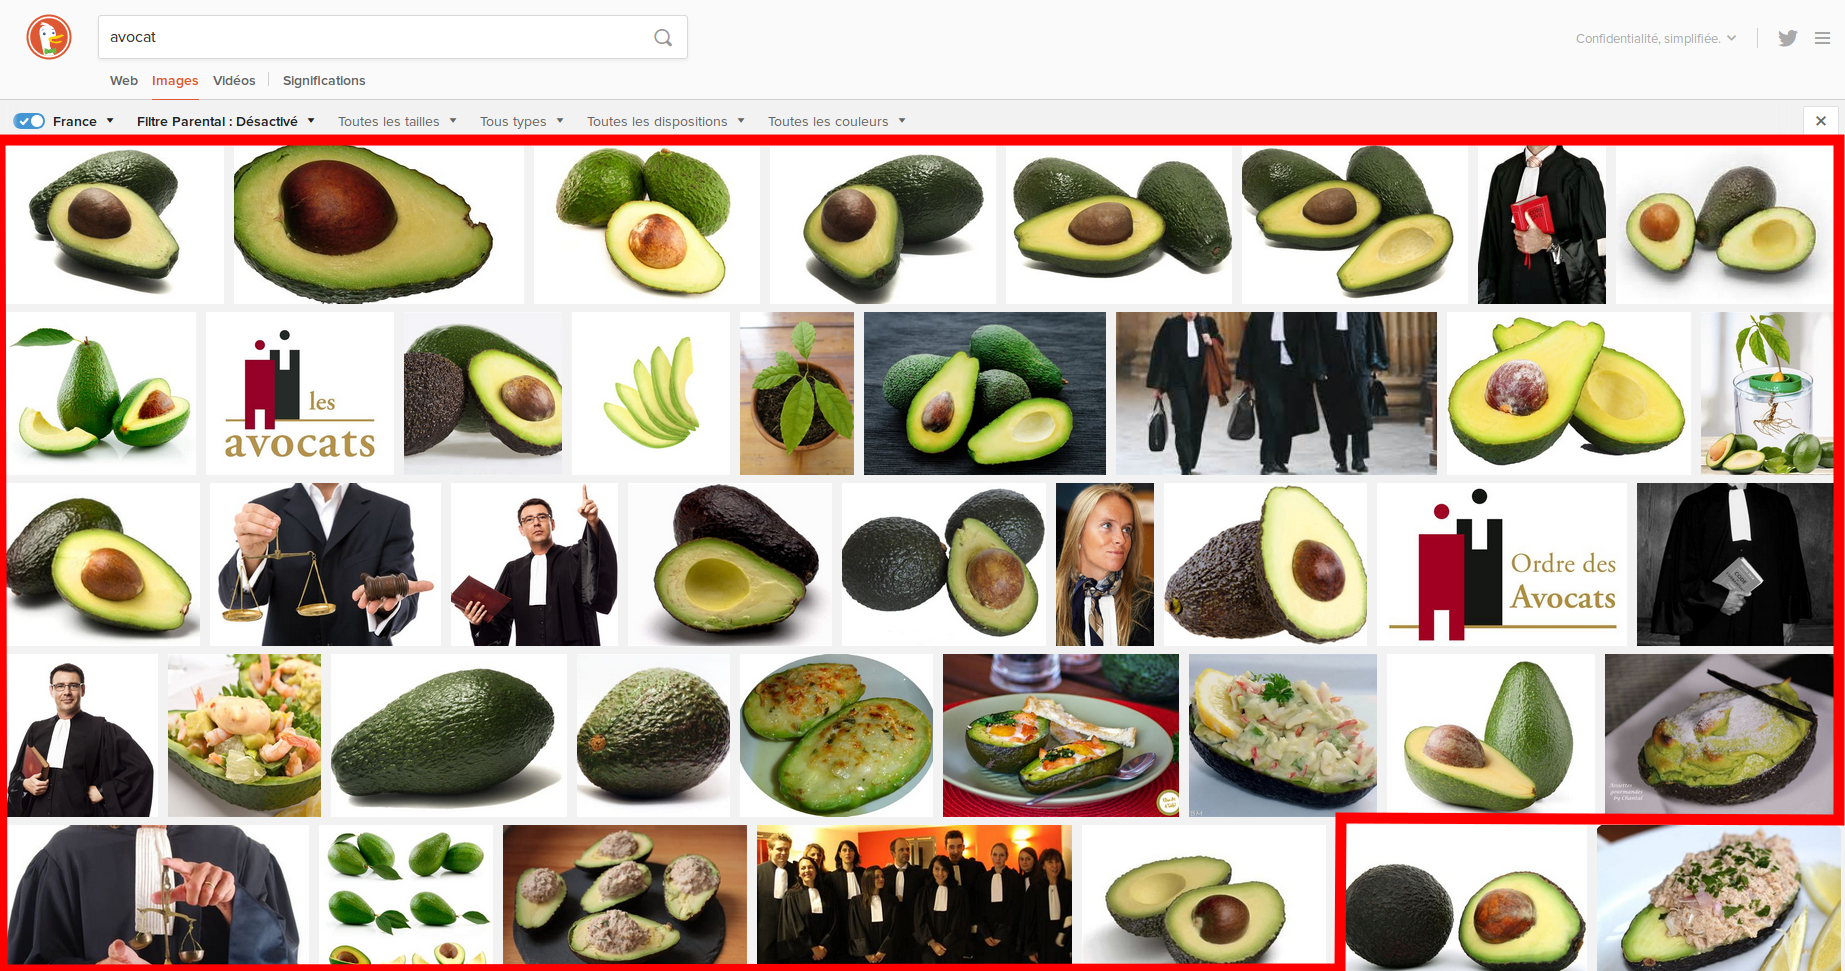
\includegraphics[width=13cm]{40_images.png}
\end{figure}

\subsection{Clustering post-retrieval}
\paragraph{K-Means}

Dans un premier temps nous allons développer une solution basée sur des méthodes de partitionnement. Notre méthode récupère une première sélection de documents qui peuvent répondre à une requête grâce à un modèle simple. 

Ici nous utilisons un modèle vectoriel qui associe à chaque document/requête un vecteur des coefficients $tfidf$ pour chaque mot qu'il contient. Nous avons au préalable enlevé les mots-creux des descriptions et nous avons effectué une \textit{stemmatization} de ces descriptions. Dans ce modèle un document est proche d'une requête s'ils contiennent les mêmes mots, notamment s'ils contiennent des mots qui apparaissent peu ailleurs.

Ensuite notre SRI réalisera un clustering des premiers documents renvoyés par notre modèle. Nous utilisons ici l'algorithme des k-moyennes. Nous faisons varier le nombre de clusters pour trouver le meilleur partitionnement, on propose d'évaluer la qualité de notre partitionnement grâce au coefficient silhouette \cite{rousseeuw87}. 
Nous avons choisi de conserver seulement les 200 premiers documents renvoyés par le modèle de base pour effectuer notre partitionnement car cela réalisait un bon compromis entre pertinence des résultats et rapidité de la réponse, pour avoir 40 résultats.

Finalement notre SRI trie les clusters selon leur proximité à la requête, et il trie les documents dans les clusters selon leur proximité à la requête. Le SRI renvoie les documents en alternant parmi les différents clusters. 

Nous allons ensuite essayer de confirmer ou d'infirmer ces choix lors de notre démarche expérimentale pour voir si notre heuristique est performante. 

\paragraph{MeanShift}
Nous utilisons un autre algorithme de clustering, MeanShift \cite{fukunuga75}, plus adapté que K-Means à notre problème.
Cet algorithme permet de partitionner un ensemble de points sans qu'on spécifie le nombre de clusters voulus, MeanShift trouve le nombre optimal de groupes.

Ainsi notre SRI effectue les mêmes étapes que pour K-Means, cependant il ne teste pas différents clusterings, ce qui accroît sa vitesse.


\subsection{Algorithme glouton} Nous allons ensuite envisager une résolution du problème de diversité en utilisant une méthode de type "glouton" \cite{zhai03}. \\

Le but de cette méthode est de maximiser la nouveauté des résultats renvoyés. En pratique on incrémente une liste de documents à renvoyer, puis à chaque itération on va chercher à renvoyer le document qui maximise la nouveauté par rapport aux documents déjà présents dans la liste.

Plus formellement on a l'algorithme suivant:

\begin{algorithm}
\caption{Algorithme glouton}
\begin{algorithmic}
\REQUIRE $U$ un ensemble de documents non-ordonnés
\REQUIRE $K$ le nombre de documents à ordonner
\REQUIRE $q$ une requête
\FOR {$i=1,2,\dots,K$} 
\STATE $d_i \leftarrow \arg\max_{d_u \in U} value(d_u;q, d_1,d_2,\dots,d_{i-1})$ 
\STATE $U \leftarrow U \backslash \left\{d_i\right\}$
\ENDFOR
\RETURN Les documents dans l'ordre $\left\{d_1, d_2,\dots, d_K\right\}$
\end{algorithmic}
\end{algorithm}

Les avantages de cet algorithme sont sa simplicité, sa potentielle rapidité car l'algorithme obtient un classement document par document, et sa flexibilité, car il est facile de changer la fonction $value$ qui est le cœur de l'algorithme. Cependant comme beaucoup d'heuristique cette méthode peut facilement trouver un optimum local plutôt qu'un optimum global.


On utilisera comme fonction $value$ la \textit{Maximal Marginal Relevance} : 
$$value_{MMR}(d_u;q,d_1,...,d_{i-1}) = \underbrace{\alpha Sim_{1}(d_u,q)}_{\text{pertinence}} - \underbrace{(1-\alpha)\max\limits_{j < i} Sim_{2}(d_u, d_j)}_{\text{divserité}}$$

Où :\\
$Sim_{1}$ et $Sim_{2}$ sont des mesures de similarités classiques, par exemple la similarité cosine (un document et une requête sont représentés par un vecteur tf-idf de termes).

\newpage
\section{Expérimentations}
\subsection{Présentation des données \textit{easyCLEF08}}
Nous avons utilisé un jeu de données appelé \textit{easyCLEF08} provenant du corpus IAPR TC-12 \cite{grubinger06} et de la vérité terrain de ce corpus \cite{arni08}. 

Ces données consistent en un ensemble de 2256 photos décrites par du texte, et un ensemble de 39 requêtes textuelles, ainsi qu'un ensemble de <<pertinences>>, des triplets $(q,d,t)$ où $q$ est la requête, $d$ est un document pertinent pour cette requête, et $t$ est le numéro du sous-thème de la requête $q$ auquel $d$ appartient.
Par exemple la requête n°2 cherche des églises avec au moins deux tours et a pour photos pertinentes des photos de Moscou (sous-thème n°1), de St-Petersburg (sous-thème n°2), etc.

\subsection{Présentation des mesures d'évaluation}
Comme en RI classique nous utilisons la précision pour évaluer la pertinence de notre SRI. Nous considérons qu'un utilisateur regarde environ 40 résultats pour une requête, c'est pourquoi nous utiliserons la métrique <<précision à 40 résultats>>, $P@40$, qui compte la proportion de documents pertinents parmi les 40 premiers résultats.

Pour mesurer la diversité des réponses renvoyées, nous utilisons une mesure appelée Cluster Recall à $n$ documents, $CR@n$, qui mesure la fraction de sous-thèmes couverts par les $n$ premiers résultats (ici $n=40$).


\subsection{Résultats du clustering post retrieval}
Nous avons évalué nos méthodes de clustering post retrieval sur un ensemble de 10 requêtes aléatoires, et nous avons comparé nos résultats à ceux de la baseline, ici un modèle vectoriel qui utilise les coefficients $tfidf$.

Nous comparons la précision à 40 documents de la baseline ("Base prec.") à la précision de notre clustering post retrieval ("PRC prec.") et nous comparons de même les Cluster Recall à 40 documents ("Base CR" et "PRC CR").

Ici nos deux modèles pour notre SRI effectuent un clustering sur les 200 meilleurs documents pour une requête, nous avons effectué plusieurs tests et c'est le meilleur compromis entre rapidité d'exécution et résultats.

Nous avons testé notre modèle sur quelques requêtes avant d'évaluer globalement ses performances, et voici l'évolution de la P@40 et du CR@40 sur une requête, avec le clustering K-Means, en fonction du nombre de clusters.

\begin{figure}[H]
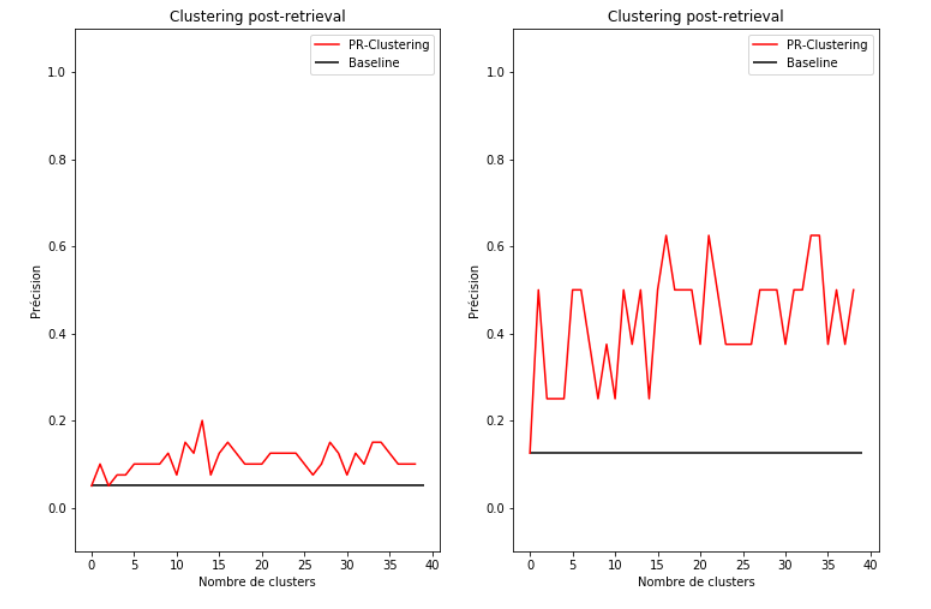
\includegraphics[scale=0.4]{img/qry11.png}
\caption{Résultats du clustering sur une requête}
\end{figure}

On voit que pour un cluster, on retrouve le résultat de la baseline, ce qui permet d'éliminer une source de bugs. 

Nous avons ensuite testé nos modèles sur une série de 10 requêtes tirées aléatoirement parmi l'ensemble disponible, afin d'évaluer les performances de notre SRI.

\begin{figure}[H]
\begin{tabular}{l*{6}{c}r}
N° requête & Base prec. & PRC prec. & Delta  & Base CR & PRC CR & Delta\\ 
\hline
   18 &    0.42   &   0.42   &   0.00 &  0.56  & 0.56  &   0.00 \\
   28 &    0.47   &   0.47   &   0.00 &  1.00  & 1.00  &   0.00 \\
   60 &    0.86   &   0.55   &  -0.31 &  1.00  & 1.00  &   0.00 \\
   16 &    0.62   &   0.57   &  -0.05 &  0.52  & 0.61  &   0.09 \\
   34 &    0.50   &   0.47   &  -0.03 &  0.57  & 0.57  &   0.00 \\
   39 &    0.57   &   0.42   &  -0.15 &  0.75  & 0.75  &   0.00 \\
   44 &    0.05   &   0.12   &   0.07 &  0.13  & 0.20  &   0.07 \\
   10 &    0.40   &   0.33   &  -0.08 &  0.17  & 0.13  &  -0.04 \\
   52 &    0.69   &   0.55   &  -0.14 &  0.71  & 0.71  &   0.00 \\
   13 &    0.28   &   0.38   &   0.10 &  0.44  & 0.56  &   0.11 \\
\hline
Moyenne  &    0.49   &   0.43   &  -0.06 &  0.59  & 0.61  &   0.02 \\
\end{tabular}
\caption{Résultats K-Means}
\end{figure}

\begin{figure}[H]
\begin{tabular}{l*{6}{c}r}
N° requête & Base prec. & PRC prec. & Delta  & Base CR & PRC CR & Delta\\ 
\hline
   18 &    0.42   &   0.42   &   0.00 &  0.56  & 0.56  &   0.00 \\
   28 &    0.47   &   0.47   &   0.00 &  1.00  & 1.00  &   0.00 \\
   60 &    0.86   &   0.86   &   0.00 &  1.00  & 1.00  &   0.00 \\
   16 &    0.62   &   0.68   &   0.05 &  0.52  & 0.57  &   0.04 \\
   34 &    0.50   &   0.50   &   0.00 &  0.57  & 0.43  &  -0.14 \\
   39 &    0.57   &   0.60   &   0.03 &  0.75  & 1.00  &   0.25 \\
   44 &    0.05   &   0.05   &   0.00 &  0.13  & 0.07  &  -0.07 \\
   10 &    0.40   &   0.40   &   0.00 &  0.17  & 0.17  &   0.00 \\
   52 &    0.69   &   0.69   &   0.00 &  0.71  & 0.71  &   0.00 \\
   13 &    0.28   &   0.25   &  -0.03 &  0.44  & 0.44  &   0.00 \\
\hline
Moyenne  &    0.49   &   0.49   &   0.00 &  0.59  & 0.59  &   0.01 \\
\end{tabular}
\caption{Résultats MeanShift}
\end{figure}

On voit que nos méthodes de clustering améliorent assez peu la baseline. En effet le clustering K-Means améliore le CR@40 de 2\% mais diminue la P@40 de 6\%, tandis que le clustering MeanShift améliore le CR@40 de 1\% et conserve la précision. 

Par ailleurs comme les requêtes ne sont pas nombreuses (39 requêtes au total dans le dataset), il peut exister une grande variance parmi les résultats de notre SRI.

Ces résultats peuvent s'expliquer par le fait que le modèle vectoriel avec les coefficients $tfidf$ est réputé être performant, ainsi il peut être difficile d'améliorer les résultats de ce modèle. C'est assez flagrant en regardant les résultats de la baseline : une précision de presque 1/2 et un CR@40 de 0,6, ce qui correspond à des bons résultats.

Nous avons utilisé ici l'algorithme K-Means classique où le seul paramètre est le nombre de clusters, que nous faisons varier à chaque requête afin de trouver le meilleur partitionnement, donc notre modèle de clustering avec K-Means ne nécessitait pas d'étude particulière de paramètre.

L'algorithme MeanShift dépend lui aussi d'un paramètre "bande-passante" pour estimer la densité des échantillons, et on peut aussi estimer ce paramètre en étudiant les données, afin d'obtenir le meilleur clustering, c'est ce que nous avons fait.

L'avantage du MeanShift est qu'il est beaucoup plus rapide que K-Means. En effet lorsque nous utilisons un clustering pour répondre à une requête, le SRI récupère 200 documents, les partitionne et renvoie un nouveau classement de 40 documents.
Le K-Means teste différents partitionnements, de 2 à 200 partitions, ce qui prend beaucoup de temps (de l'ordre de 4 secondes pour obtenir un nouveau classement), comparé au MeanShift qui étudie d'abord les données et qui effectue ensuite un clustering (de l'ordre de 200 ms).

\section{Conclusion}

Nous avons vu que sur le corpus easyCLEF08 nos modèles de clustering n'étaient pas beaucoup plus performants que le modèle de base vectoriel avec $tfidf$.

Nous avons remarqué que beaucoup de requêtes contenaient non seulement la requête en elle-même (<< church with more than two towers >>), mais aussi une description plus détaillées des résultats attendus : << Relevant images will show a church, cathedral or a mosque with three or more towers... >> ou pour une autre requête << Non-religious statues like war memorials or monuments are not relevant. >>. Cela pose un problème car notre modèle de base pour le clustering suppose que chaque mot de la requête est << voulu >>, notre modèle ne comprend pas la négation, il va essayer de trouver des documents qui contiennent les mêmes mots que la requête, même si cela va à l'encontre de ce que l'utilisateur voulait. 
Ainsi il faudrait utiliser un modèle plus subtil qui comprendrait ce que veut un utilisateur et ce qu'il ne veut pas. Cela est possible en utilisant d'autres modèles du traitement automatique du langage.

\begin{thebibliography}{9}
\bibitem{rousseeuw87}
\textit{Silhouettes: A graphical aid to the interpretation and validation of cluster analysis},
Peter J.Rousseeuw

\bibitem{fukunuga75}
\textit{The Estimation of the Gradient of a Density Function, with Applications in Pattern Recognition}, Fukunaga, Keinosuke, Hostetler

\bibitem{zhai03}
\textit{Beyond Independent Relevance: Methods and EvaluationMetrics for Subtopic Retrieval}, Zhai, Cohen, Lafferty

\bibitem{grubinger06}
\textit{ImageCLEF 2006
Text and/or Content-Based Cross Language Image Retrieval}, Grubinger et al.

\bibitem{arni08}
\textit{Overview of the ImageCLEFphoto 2008  
Photographic Retrieval Task}, Arni et al.
\end{thebibliography}


\end{document}